\documentclass[oneside,14pt]{extarticle}
\usepackage[utf8]{inputenc}
\usepackage[english,ukrainian]{babel}
\usepackage[T1]{fontenc}
\usepackage{amssymb,amsfonts,amsmath,amsthm,mathtext,textcomp}

\usepackage[includehead, headsep=0pt, footskip=0pt, top=2cm, bottom=2cm, left=2.5cm, right=1cm]{geometry}
\usepackage{indentfirst}
\usepackage[onehalfspacing]{setspace}
\usepackage[headings]{fancyhdr}
\usepackage{etoolbox}
\usepackage{flafter}
\usepackage{listings}
\usepackage{graphicx}
\usepackage{float}
\usepackage[center]{titlesec}
\usepackage{hyperref}
\usepackage{array}
\fancyhf{}
\renewcommand{\headrulewidth}{0pt}
\fancyhead[R]{\thepage}
\pagestyle{fancy}
\fancypagestyle{plain}{%
	\fancyhf{}
	\fancyhead{}
	\fancyfoot{}
	\fancyhead[RO]{\thepage}
	\fancyhead[LE]{\thepage}
	\renewcommand{\headrulewidth}{0pt}
	\renewcommand{\footrulewidth}{0pt}
}
\lstset{breaklines=true,}
\graphicspath{ {./pictures} }
\counterwithin{figure}{section}
\titlelabel{\thetitle.\quad}
\renewcommand*{\thesection}{Розділ~\arabic{section}}
\renewcommand*{\thesubsection}{\roman{subsection}}
\renewcommand{\thefigure}{\arabic{section}.\arabic{figure}}
\usepackage{tocloft}
\setlength{\cftsecnumwidth}{5em}
\setlength\parindent{1.25cm}
\usepackage{enumitem}

\begin{document}
\begin{titlepage}
	\begin{center}
		Національний університет <<Львівська політехніка>>\\
		Кафедра програмного забезпечення
		
		\vspace{40pt}
		\textbf{\LARGE КУРСОВА РОБОТА}\\
		{\large
		\textbf{з дисципліни <<Бази даних>>}\\
		на тему:\\
		<<Інформаційна система для ...>>
		}
		\vspace*{40pt}
		
		\begin{flushright}
		    \begin{minipage}{0.6\textwidth}
		        \underline{Виконав}:\\
                Стедент спеціальності 121\\
			    <<Інженерія програмного забезпечення>>\\
			    групи ПЗ-32\\
			    Коваленко Д.М.
			    \bigbreak
			    
			    \underline{Керівник}:\\
			    асистент кафедри програмного забезпечення\\
			    Білоіваненко М.В.
			    \bigbreak
			    
			    \underline{Оцінка}:\\
			    Національна шкала \rule{6.35cm}{0.15mm}\\			
			    Кількість балів \rule{2cm}{0.15mm} Оцінка ECTS \rule{2cm}{0.15mm}
			    \bigbreak
            \end{minipage}
		\end{flushright}
		\vspace{40pt}
		Члени комісії \hspace{1.9cm} \rule{3cm}{0.15mm} \hspace{1cm} Білоіваненко М.В.\\
		{\small\vspace{-5pt}(підпис)}\\
		\hspace{2.65cm}\hspace{1.9cm}  \rule{3cm}{0.15mm} \hspace{1cm} Цимбалюк Т.М.\\
		{\small\vspace{-5pt}(підпис)}\\
		
		\vspace{\fill}
		Львів — 2024
	\end{center}
\end{titlepage}
\setcounter{page}{2}
\tableofcontents
\newpage

\section{Аналіз предметної області та постановка завдання}
\subsection{Опис предметної області}
% Актуальність
З кожним днем мобільність населення постійно зростає, транспортна інфраструктура розвивається, потреба у вдосконаленні та оптимізації процесів управління перевезеннями постійно росте. Компанії, які здійснюють регулярні перевезення, стикаються з великою кількістю даних, складних розрахунків і потребують ефективних інструментів для керування цими процесами. Розробка інформаційної системи для компанії з регулярних перевезень стає необхідністю для оптимізації витрат, підвищення якості обслуговування та конкурентоспроможності.

\begin{list}{-}{Специфікація важливих понять:}
\item Зупинка - статичне місце, де зупиняться транспорт для посадки та висадки пасажирів.
\item Квиток - карта, видана пасажиру, що має баланс.
\item Технічне обслуговування транспортних засобів - заправка, зміна шин, загальний огляд, прибирання, тощо.
\end{list}

% Встановлення обсягів аналізу теми
Аналіз предметної області буде обмежений на даних про перевезення пасажирів автобусами, не включаючи трамваї, метро, залізничний транспорт, пароми, канатні дороги, гондоли, фунікулери.

\subsection{Вимоги до обробки даних}
% Опис актуальних бізнес процесів
Бізнес-процеси компанії з регулярних перевезень пасажирів включають ряд дій та етапів, які забезпечують ефективну організацію та функціонування пасажирських перевезень. Компанія визначає регулярні маршрути, графіки руху та зупинки для пасажирських транспортних засобів. Це включає вибір оптимальних маршрутів, розподіл транспортних засобів та встановлення годин руху. Призначення водіїв на кожен транспортний засіб.

% Опис накопичення та аналізу даних
Для ефективного управління пасажирськими перевезеннями необхідно накопичувати та аналізувати різноманітні дані. Це включає в себе збір інформації про рух транспортних засобів, кількість пасажирів на кожній зупинці, реєстрацію квитків та транзакцій, а також звіти про витрати і доходи. Аналіз цих даних допоможе виявити патерни в руху пасажирів, визначити популярні маршрути та години, забезпечити достатню кількість транспортних засобів для попиту, а також виявити ефективність роботи водіїв та рейсів.

% Деталізація інформаційних структур
База даних для інформаційної системи компації з регулярних перевезень повинна містити наступні ключові сутності:
\begin{itemize}
\item Зупинка - інформація про місце, призначене для посадки та висадки пасажирів.
\item Маршрут - послідовність зупинок, які обслуговує певний транспортний засіб.
\item Транспортний засіб - засіб перевезення пасажирів, який обслуговує певний маршрут.
\item Водій - особа, яка керує транспортним засобом під час перевезення пасажирів.
\item Квиток - інформація про проїзну карту видану пасажиру.
\item Транзакція - запис, що фіксує факт використання квитка пасажиром на конкретному маршруті та у певний час.
\item Розклад руху - перелік часу прибуття та відправлення транспортного засобу на кожній зупинці певного маршруту.
\end{itemize}

\subsection{Постановка завдання}
% Перелік необхідних функцій інформаційної системи
Інформаційна система для компанії з регулярних перевезень повинна мати ряд ключових функцій, що забезпечують ефективне управління та оптимізацію бізнес-процесів. Перш за все, система повинна забезпечувати зберігання та оновлення інформації про перевезення пасажирів, доступні маршрути та транспортні засоби.

З урахуванням періодичної природи бізнесу, система має підтримувати пов’язані з часом події, такі як регулярні рейси, їх час та тривалість, а також фіксувати дані про пасажирів і операції щодо їх перевезення. Вона також повинна забезпечувати можливість аналізу цих даних для виявлення тенденцій та оптимізації ресурсів.

\begin{list}{•}{Інформаційна система для компанії з регулярних перевезень повинна мати наступні функції:}
    \item Довготривале зберігання та оновлення даних про перевезення пасажирів, транспортні засоби та маршрути.
    \item Можливість внесення нових даних та редагування існуючих з урахуванням обмежень цілісності.
    \item Функції сортування, вибірки та пошуку інформації для аналізу та оптимізації бізнес-процесів.
    \item Представлення даних у зручній табличній формі для зручного аналізу та використання.
    \item Інтерактивний інтерфейс користувача, що відповідає логіці бізнес-процесів компанії.
\end{list}
\newpage

\section{Розробка моделей зберігання даних}
\subsection{Концептуальне проектування}
% Взаємозв’язки та характеристики понять, що описані в базі даних
Основними структурами інформаційної системи для компанії з регулярних перевезень визначено наступні компоненти:
\begin{itemize}
\item Зупинка
\item Маршрут
\item Розклад
\item Транспортний засіб
\item Водій
\item Квиток
\item Транзакція
\item Технічне обслуговування
\item Види пільг для квитка
\end{itemize}

Основними зв'язками між переліченими сутностями можна визначити наступні відношення:
\begin{itemize}
\item Маршрут - зупинка (many to many): маршрут може містити кілька зупинок, кожна зупинка може належати кільком маршрутам.
\item Квиток - транзакція (one to many): кожен квиток може бути пов'язаний з багатьма транзакціями, транзакція може мати лише один асоційований квиток.
\item Водій - транспортний засіб (one to one): кожен водій може бути пов'язаний лише з одним транспортним засобом.
\item Транспортний засіб - маршрут (one to one): кожен транспортний засіб може бути пов'язаний лише з одним маршрутом.
\end{itemize}

\subsection{Вимоги до системи накопичення даних}
% Оцінка обсягів даних
Обсяги даних, що будуть зберігатися в інформаційній системі для компанії з регулярних перевезень, залежать в першу чергу від масштабів та рівня розвитку мережі транспортного сполучення. Беручи до уваги розмір первинних історичних даних для міста Мельбурн (Австралія), можна припустити, що база даних буде містити в середньому кілька сотень маршрутів, кілька тисяч зупинок та близько мільйона записів про розклад руху, при цьому необхідно зберігати інформацію про тисячу транспортних засобів та водіїв, а також обробляти близько трьох мільйонів транзакцій від двох мільйонів пасажирів щодня.

% Частота додавання
Очевидно найзатребуванішими ресурсами бази даних для додавання, буде інформація про транзакції та пасажирів. Іншим затребуваним ресурсом для додавання може бути інформація про обслуговування транспортних засобів, особливо під час початку або завершення робочого дня, коли проводиться технічне обслуговування транспортних засобів.

Для читання найзатребуванішими запитами буде отримування розкладу руху для пасажирів та деталей маршруту для водія.

% Очікувані запити та вибірки
TODO

% Обмеження доступу та ін.
Для обмеження доступу користувачів було створено три основні ролі - \textit{passenger}, \textit{driver}, \textit{manager}.

\begin{itemize}
\item \textit{passenger} - має доступ до отримання розкладу руху на вказаній зупинці, та можливість пошуку маршрутів між двома зупинками. Такод має право створювати транзакції.
\item \textit{driver} - може додавати дані до таблиці \textit{maintenance}, та отримувати дані про поточний маршрут.
\item \textit{manager} - має повний доступ до всіх даних.
\end{itemize}

\subsection{Логічне проектування схеми бази даних}
% Домени
Основними доменами схеми бази даних передбачено дані для пасажирів (розклад руху, квитки, транзакції), дані для водіїв (розклад руху, записи про технічне обслуговування транспортних засобів) та менеджерів (управління розкладом руху, маршрутами, тощо).

% Таблиці
База даних для предметної області складається з наступних структур:
\begin{itemize}
\item Таблиця \textit{Stop} містить дані про назву та розміщення (широта, довгота) місць, де транспорт зупиняється для посадки та висадки пасажирів.
\item Таблиця \textit{Route} містить дані про коротку та повну назву маршрутів руху транспорту.
\item Таблиця \textit{Driver} містить дані про ім'я водія та ідентифікаційний номер транспортного засобу, що призначений водієві.
\item Таблиця \textit{Vehicle} містить дані про номерний знак транспортого засобу та кількість місць для пасажирів.
\item Таблиця \textit{Maintenance} містить дані про ідентифікаційний номер транспортного засобу та водія, опис, вартість та час проведення обслуговування.
\item Перелічуваний тип \textit{Ticket\_discount} вказує на вид пільги квитка, містить варіанти \textit{student}, \textit{elder}, \textit{veteran}.
\item Таблиця \textit{Ticket} містить дані про тип пільги, якщо така існує, та доступний баланс.
\item Таблиця \textit{Transaction} містить дані про ідентифікаційний номер квитка, маршруту, транспортного засобу, зупинки на якій відбулась посадка пасажира, зупинка на якій відбулась висадка пасажира, вартість проїзду  та час.
\item Таблиця \textit{Schedule} містить дані про ідентифікаційний номер маршруту, зупинки, та час прибуття і відправлення.
\item Таблиця \textit{Route\_stops} містить дані про ідентифікаційний номер маршруту, зупинки та порядковий номер зупинки на маршруті.
\item Таблиця \textit{Route\_vehicles} містить дані про ідентифікаційний номер маршрутів та транспортних засобів.
\end{itemize}

\subsection{Реалізація процедур бізнес-логіки}
% Тригери
TODO

% Процедури
Для реалізації бізнес-логіки реалізовано наступні процедури:
\begin{itemize}
\item \textit{new\_transaction} - інкапсулює логіку створення нової транзакції. Виконує валідацію вхідних даних відповідно до обмежень цілісності бази даних, виконує списання коштів з рахунку квитка, та створює новий запис у таблиці транзакцій.
\end{itemize}

% Функції
Для реалізації бізнес-логіки реалізовано наступні функції:
\begin{itemize}
\item \textit{next\_stop} - повертає назву наступної зупинки після вказаної на маршруті, та час, який залишається до прибуття.
\item \textit{search\_stop} - повертає зупинки, назва яких частково співпадає з аргументом.
\item \textit{search\_route} - повертає маршрути, назва яких частково співпадає з аргументом.
\end{itemize}

% Представлення
Для реалізації бізнес-логіки реалізовано наступні представлення:
\begin{itemize}
\item \textit{routes\_with\_stops} - повертає маршрути які містять у собі дві вказані зупинки.
\item \textit{arrival\_with\_stops\_in} - повертає час, що залишається до прибуття до вказаної зупинки, та напрямок руху транспорту на вказаній зупинці.
\end{itemize}

\newpage

\section{Розробка програмного коду}
\subsection{Обґрунтування обраної архітектури}
% Тип
Для розробки інформаційної системи для компанії з регулярних перевезень було обрано клієнт-серверну архітектуру, що дозволить абстрагуватися над реалізацією інтерфейсу користувача, що буде корисно для підтримки різноманітних форматів взаємодії з користувачем. В реальних умовах це дозволить створити мобільний додаток для пасажирів, вбудовану систему для водіїв та додаток для персонального комп'ютера для менеджера.

% Мова програмування
Для реалізації серверної частини інформаційної системи для компанії з регулярних перевезень було обрано мову програмування \textit{Go}. Завдяки своїй простоті цей вибір дозволить швидко створити прототип системи. А завдяки швидкості виконання цей вибір дозволить зосередитись на створенні нового функціоналу системи замість оптимізації існуючого.

% Система баз даних
Для реалізації бази даних інформаційної системи для компанії з регулярних перевезень було обрано \textit{PostgreSQL}, що завдяки своїй популярності та зрілості дозволить швидко створити необхідний функціонал.

% Формати
Для передачі інформації з серверу на клієнт було використано формат даних \textit{JSON}.

% Протоколи
TODO

\subsection{Структурна модель інформаційної системи}
TODO Програмна модель інформаційної системи для компанії з регулярних перевезень складається з наступних

\subsection{Призначення модулів та компонентів системи}
TODO

\subsection{Особливості реалізації та елементи інтерфейсу}
TODO

\newpage

\section{Наповнення бази даних}
\subsection{Опис джерела історичних даних}
Джерело історичних даних описує мережі громадського транспорту 25 міст по всьому світу в кількох простих у використанні форматах даних. Ці формати даних включають списки меж мережі, тимчасові списки мережевих подій, бази даних SQLite, файли GeoJSON і сумісні ZIP-файли General Transit Feed Specification (GTFS).

Вихідні дані для створення цих мереж були опубліковані агентствами громадського транспорту у форматі даних GTFS. Для створення витягів мережевих даних для кожного міста вихідні дані були відібрані на наявність помилок, відфільтровані просторово й у часі та доповнені пішохідними відстанями між зупинками громадського транспорту за допомогою даних OpenStreetMap.

Для виконання роботи були використані дані для міста Мельбурн (Австралія), що складаються з 467 маршрутів, 19649 зупинок, 2714796 записів про розклад руху.

\subsection{Опис процесів генерації тестових даних}
Тестові дані генеруються за допомогою бібліотеки Faker для Python та SQL команд з використанням функції \textit{random()}, після чого адаптуються до реляційних відношень та обмежень цілісності бази даних. 

Випадковим чином були згенеровані дані для наступних таблиць: \textit{Vehicle} (1500 записів), \textit{Driver} (2000 записів) \textit{Ticket} (1000 записів), \textit{Transaction} (100000 записів), \textit{Maintenance} (1000 записів).

\subsection{Трансформація та первинне завантаження даних}
Завантаження первинних історичних даних з мережі, запуск серверу бази даних, додавання рядків після створення відповідних таблиць та відношень реалізована в контейнеризованому оточенні за допомогою \textit{podman}, що дозволяє отримати готову до роботи, заповнену інформацією базу даних на будь якій системі за лічені хвилини.

Джерело первинної інформації містить багато додаткових даних, зокрема інформація про маршрути у форматі \textit{GEOjson}, що дозволяє переглядати їх за допомогою технології OpenStreetMap. Тому для отримання необхідних даних для опису предметної області були використані різноманітні шляхи видобування інформації, зокрема: 
\begin{itemize}
\item Перенесення даних з \textit{SQLite} до \textit{PostgreSQL} за допомогою перетворення даних у формат \textit{csv} та внесення в базу даних за допомогою команди \textit{copy}.
\item Вибірка необхідних даних з існуючих таблиць та їх перетворення до необхідного формату.
\end{itemize}

\newpage

\section{Функціональні можливості для користувача}
\subsection{Опис інтерфейсу у відповідності до бізнес-процесів}
Інтерфейс користувача дозволяє авторизуватися використовуючи логін та пароль, та, залежно від ролі користувача - виконувати різні дії над даними відповідно до бізнес-процесів.

\begin{figure}[H]
\centering
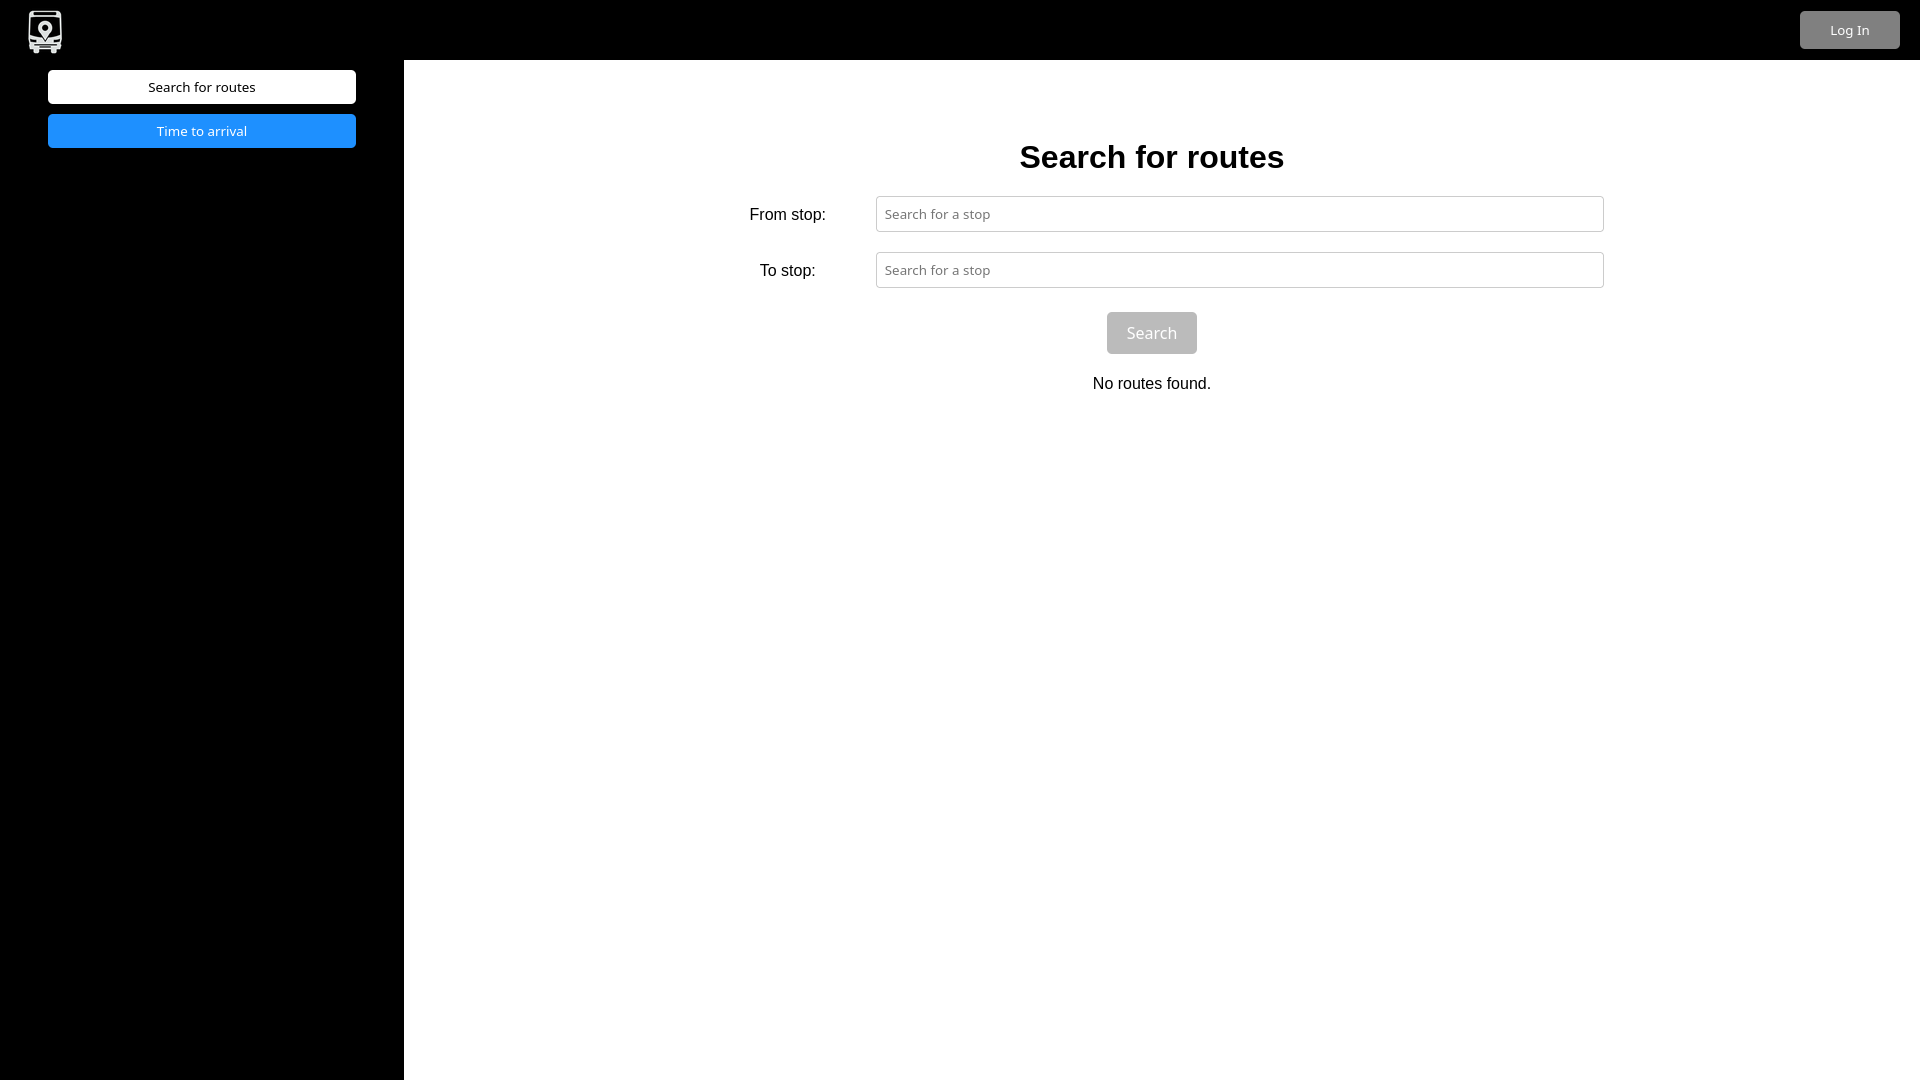
\includegraphics[scale=0.25]{1}
\caption{Сторінка авторизації.}
\end{figure}

Користувачі, авторизовані з роллю \textit{passenger}, мають можливість знайти маршрут між двома вказаними зупинками та отримати час до прибуття транспортного засобу на вказану зупинку на вказаному маршруті.

\begin{figure}[H]
\centering
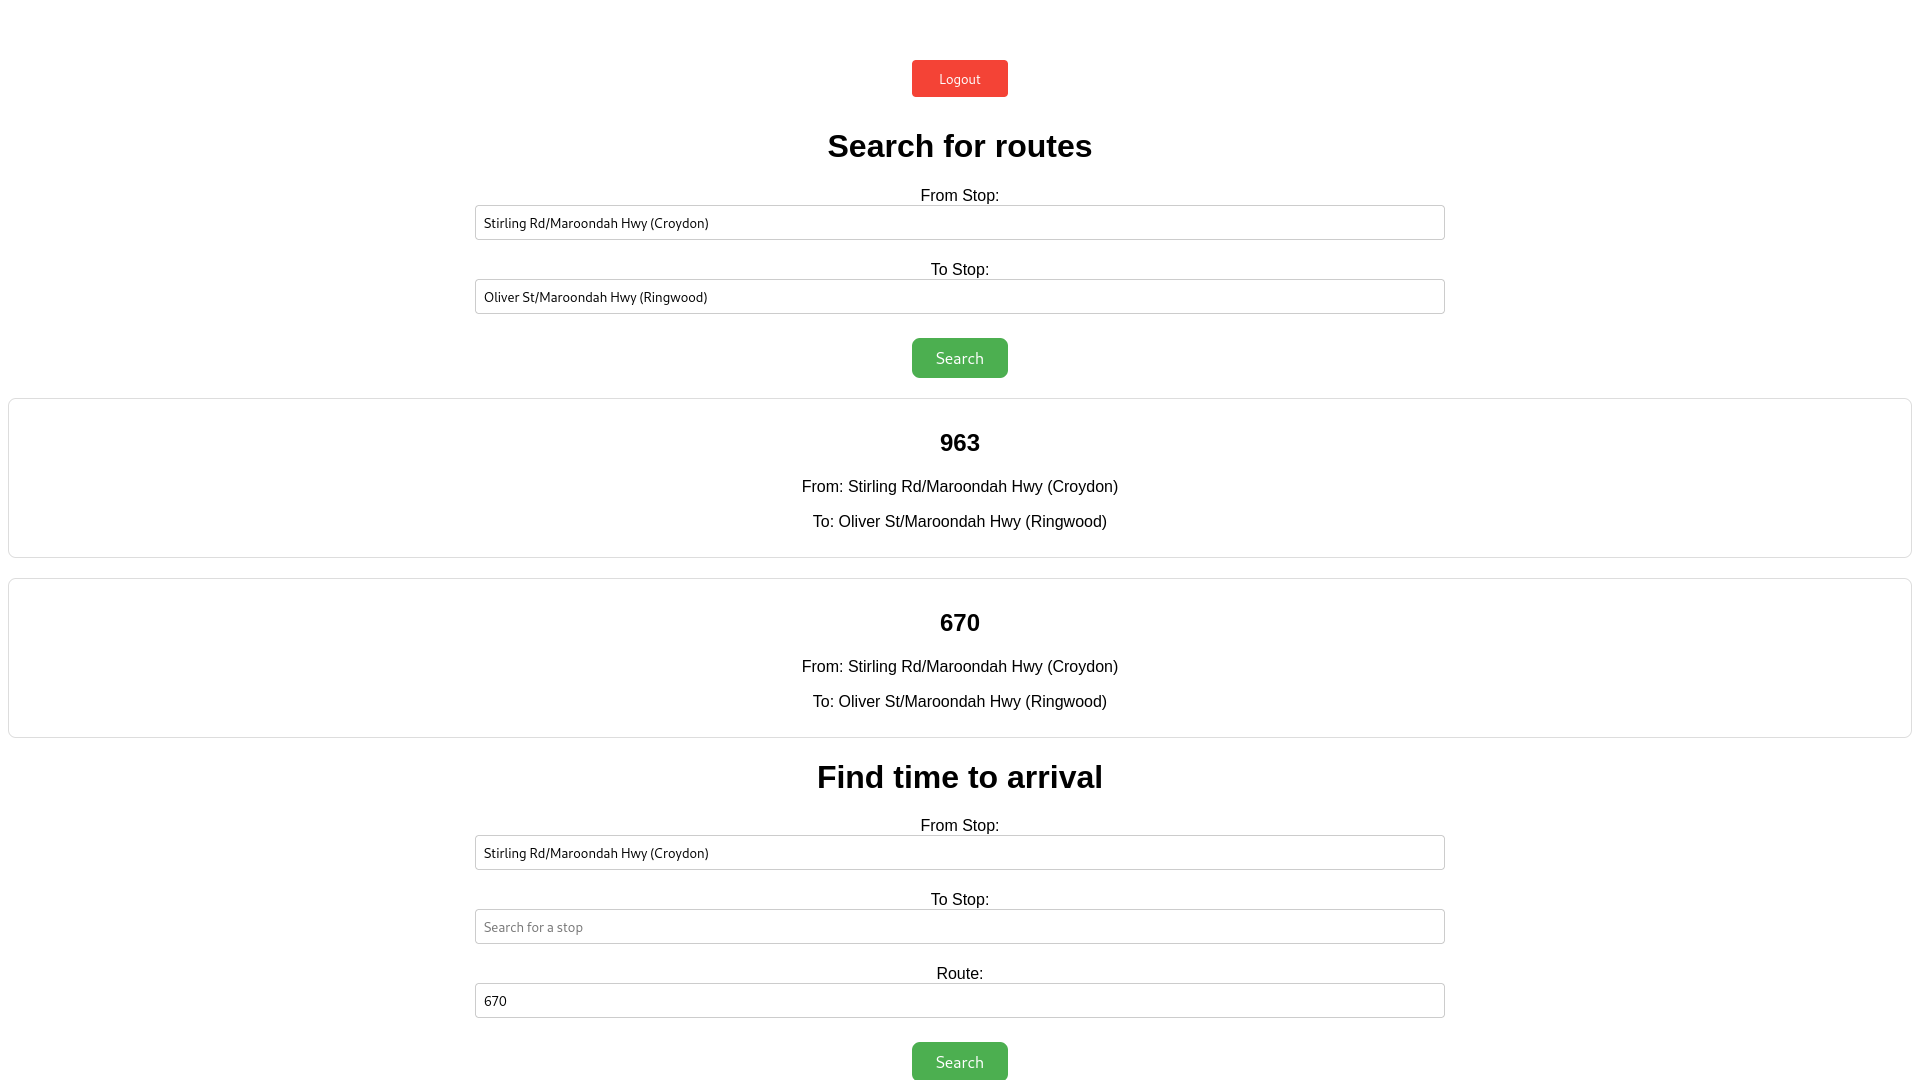
\includegraphics[scale=0.25]{2}
\caption{Пошук маршрутів між вказаними зупинками.}
\end{figure}

\begin{figure}[H]
\centering
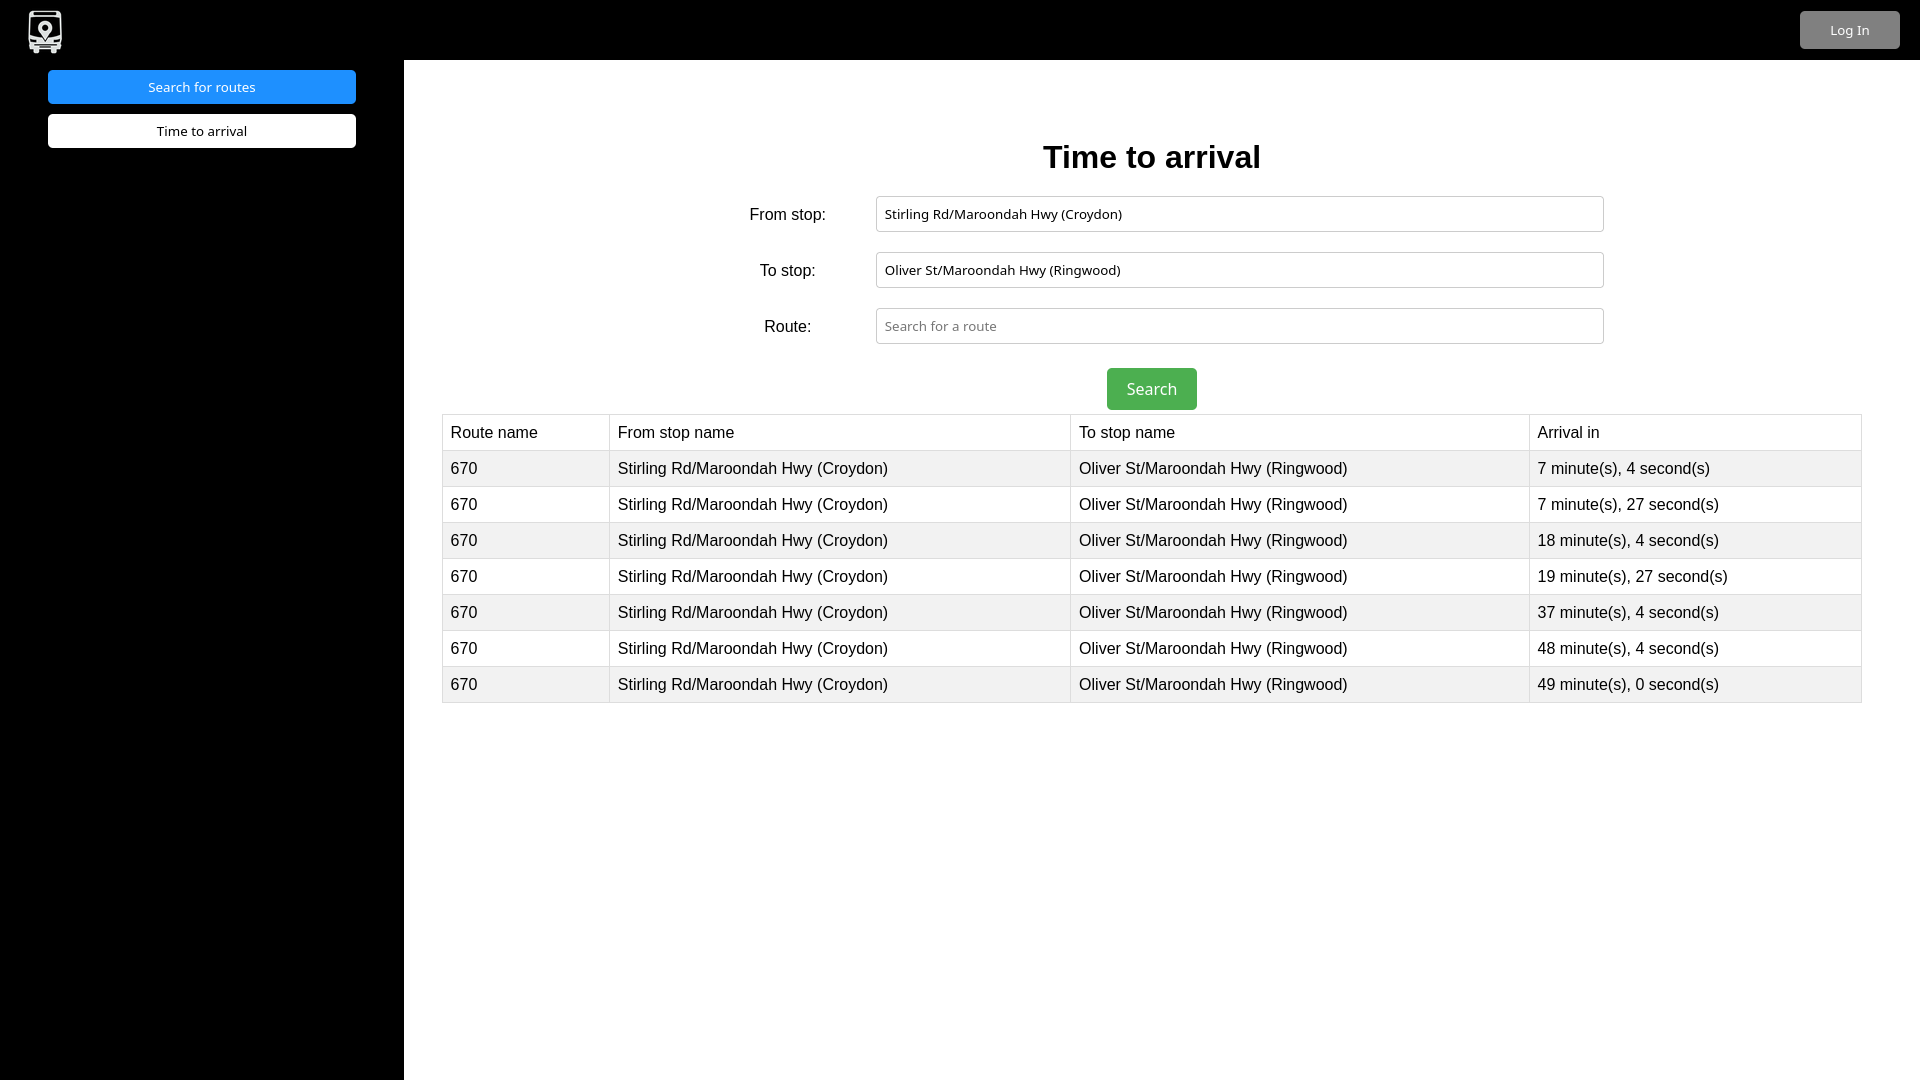
\includegraphics[scale=0.25]{3}
\caption{Отримання часу прибуття транспортного засобу на вказану зупинку на вказаному маршруті.}
\end{figure}

Користувачі, авторизовані з роллю \textit{driver}, мають можливість внести запис про технічне обслуговування, та отримати деталі маршруту.

\begin{figure}[H]
\centering
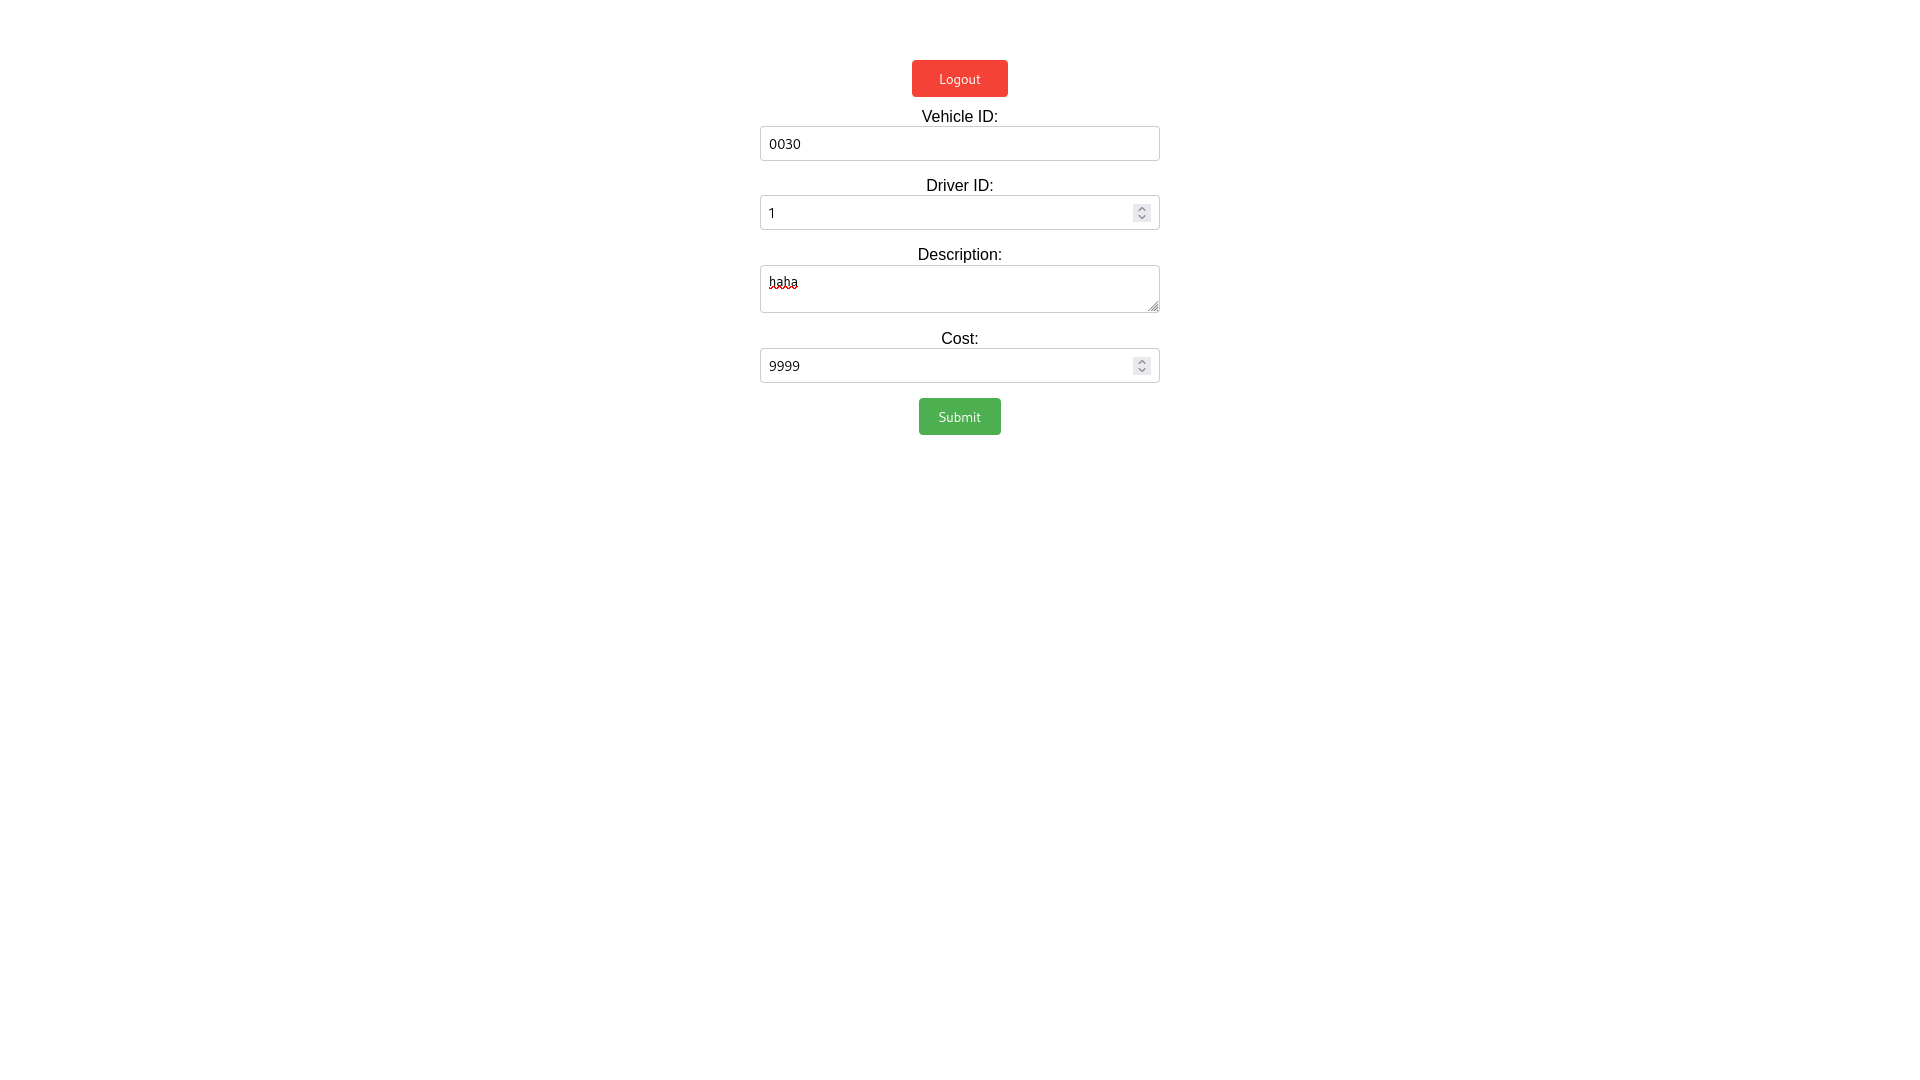
\includegraphics[scale=0.25]{4}
\caption{Внесення запису про технічне обслуговування транспортного засобу.}
\end{figure}

Користувачі, авторизовані з роллю \textit{manager}, мають можливість експортувати дані у форматі \textit{JSON}, та призначати водіїв на маршрути.

\begin{figure}[H]
\centering
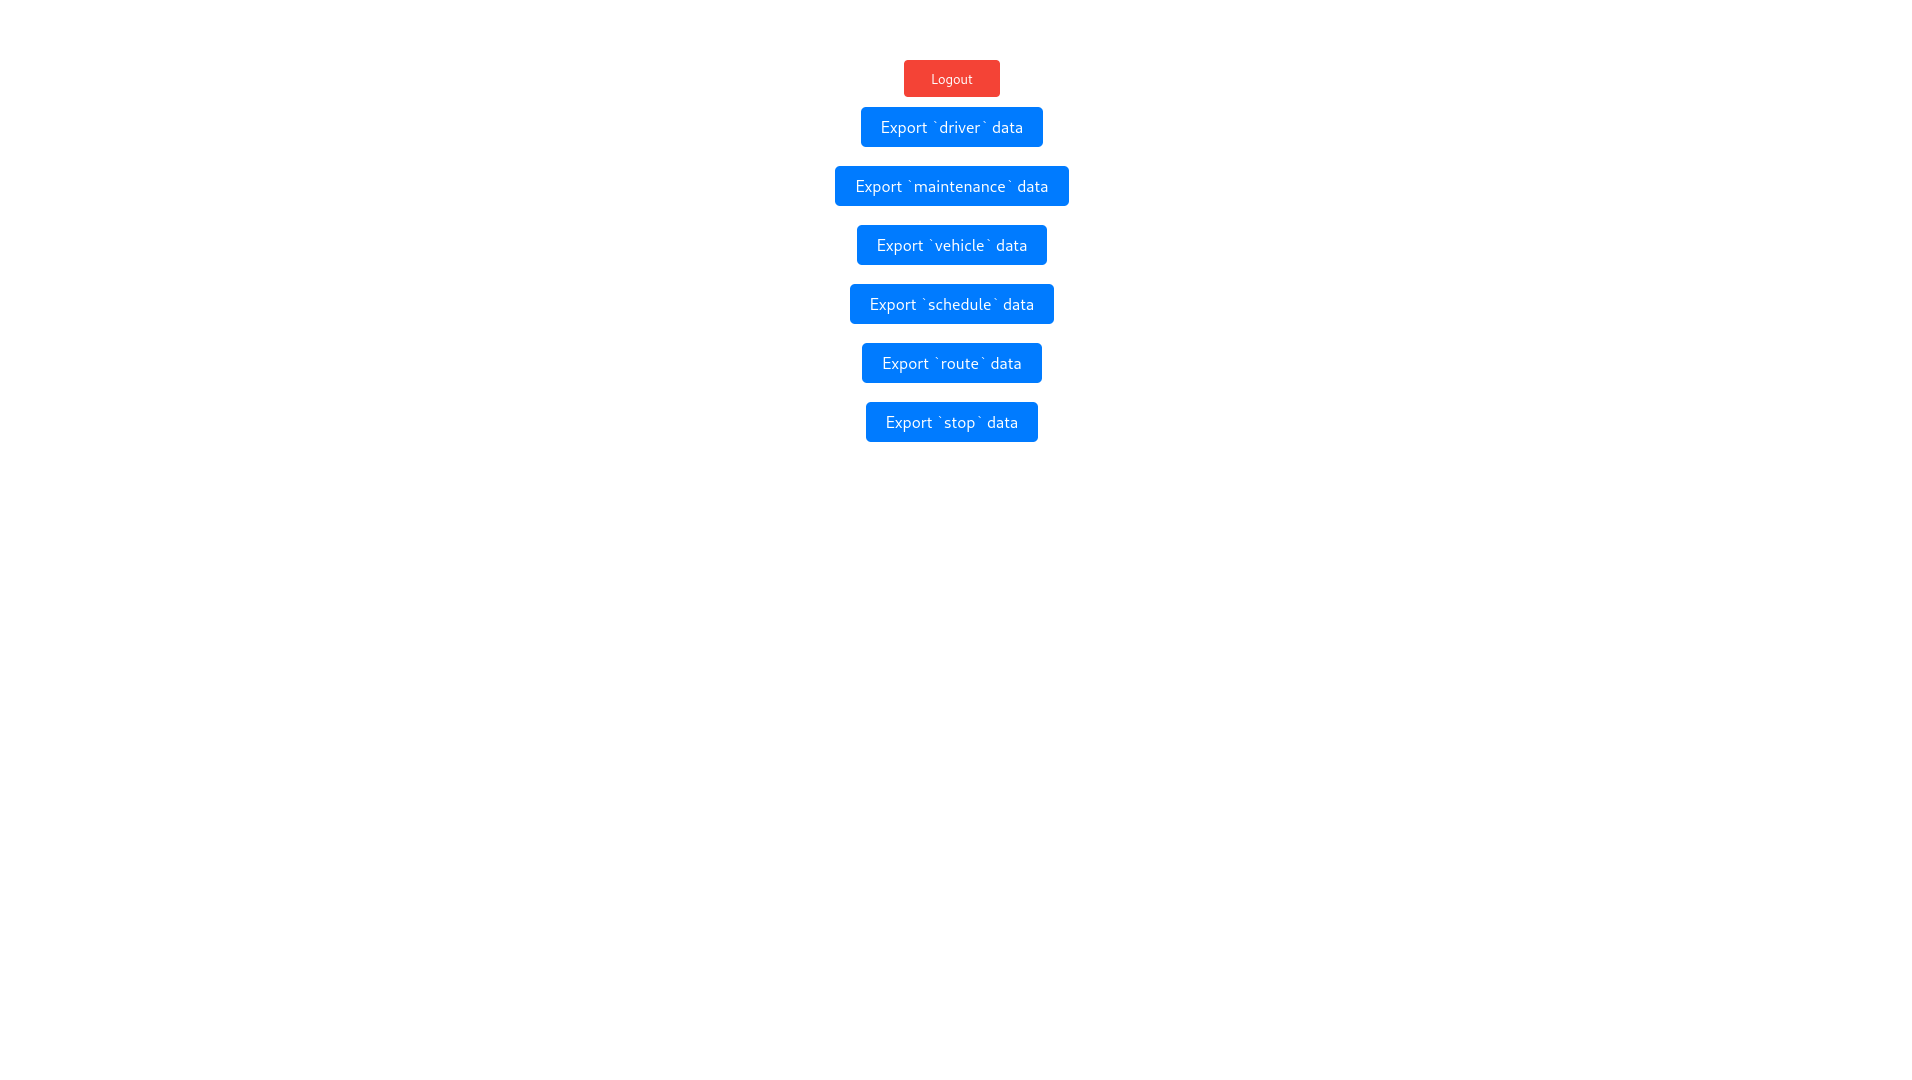
\includegraphics[scale=0.25]{5}
\caption{Експортування різноманітних даних.}
\end{figure}

\subsection{Засоби аналітичного представлення даних}
TODO

\subsection{Засоби експорту даних}
% Обмеження
TODO

% Формат файлу
TODO

\subsection{Засоби програмного інтерфейсу}
TODO

\newpage

\section{Висновки}
\subsection{Встановлені недоліки}
TODO

\subsection{Перспективи покращення}
TODO

\newpage

\section{Список літератури}
\href{https://www.researchgate.net/publication/325161554_A_collection_of_public_transport_network_data_sets_for_25_cities}{https://www.researchgate.net/publication/325161554\_A\_collection\_of\_public...}

TODO

\newpage

\section{Додатки}
\subsection{Скрипт створення бази даних та завантаження історичних даних}
{\fontsize{8pt}{8pt}\selectfont\lstinputlisting{import.sh}}

\subsection{Інший програмний код}
Файл \textit{main.go}
{\fontsize{8pt}{8pt}\selectfont\lstinputlisting{src/main.go}}

Файл \textit{models.go}
{\fontsize{8pt}{8pt}\selectfont\lstinputlisting{src/models/models.go}}

\subsection{Інший код створених моделей}
TODO

\end{document}
